% Created 2020-12-01 Tue 15:09
% Intended LaTeX compiler: pdflatex
\documentclass[number]{elsarticle}

\usepackage[utf8]{inputenc}
\usepackage[T1]{fontenc}
\usepackage{graphicx}
\usepackage{grffile}
\usepackage{longtable}
\usepackage{wrapfig}
\usepackage{rotating}
\usepackage[normalem]{ulem}
\usepackage{amsmath}
\usepackage{textcomp}
\usepackage{amssymb}
\usepackage{capt-of}
\usepackage{hyperref}
\usepackage{wasysym}
\usepackage{gensymb}
\usepackage{lipsum}

\begin{document}

\begin{frontmatter}	
  \title{The KOALA experiment for (anti)proton-proton elastic scattering}
  \date{\today}

  \author[ikp]{Yong Zhou\corref{cor}}
  \ead{y.zhou@fz-juelich.de}
  \author[ikp]{Huagen Xu}
  \author[ikp,bochum]{James Ritman}

  % cluster target group
  \author[muenster]{Alfons Khoukaz}
  \author[muenster]{Lukas Leßmann}
  \author[muenster]{Benjamin Hetz}
  \author[muenster]{Christopher Fritzsch}

  % vacuum & mechanics group
  \author[ikp]{Ulf Bechstedt}
  \author[ikp]{Jürgen Böker}
  \author[ikp]{Steffen Quilitzsch}
  \author[ikp]{Nils Demary}

  % beam group

  % electronics group

  % other collaborators

  \cortext[cor]{Corresponding author}
  \fntext[fn1]{Present address: Institute of Modern Physics, Chinese Academy of Sciences, Lanzhou, 730000, China}
  \fntext[fn2]{Present address: GSI Helmholtzzentrum für Schwerionenforschung GmbH, Darmstadt, 64291, Germany}

  \address[ikp]{Institut für Kernphysik, Forschungszentrum Jülich, Jülich, 52425, Germany}
  \address[muenster]{Institut für Kernphysik, Universität Münster, Münster, 48149, Germany}
  \address[zea]{Zentralinstitut für Engineering, Elektronik und Analytik, Forschungszentrum Jülich, Jülich, 52425, Germany}
  \address[bochum]{Ruhr-Universität Bochum, Bochum, 44780, Germany}


  \begin{abstract}
    % Cross section data of (anti)proton-proton elastic scattering is important
    % for the study of nuclear forces and also provides necessary ingredients in
    % the modeling of meson production and other nuclear reactions at intermediate energies.

    % A good understanding of the nucleon-nucleon interaction is one of the principal
    % goals of nuclear and hardon physics.

    The KOALA experiment is designed to measure the differential cross section
    of (anti)proton-proton elastic scattering over a wide range of four-momentum
    transfer squrared $0.0005 < |t| < 0.1$ $(GeV/c)^2$.
    % The forward scattering parameters and the absolute luminosity can be deduced
    % by analyzing the characteristic shape of the differential cross section spectrum.
    It's a fixed-target experiment with an internal hydrogen cluster target.
    The wide range is achieved by measuring the total energy of the recoil proton with a
    position-sensitive recoil detector.
    A forward detector is used to measure the coincidence scattering particle to
    suppress the background events at small recoil angle.
    KOALA aims to be commissioned at COSY for proton-proton measurement and at
    FAIR-HESR for antiproton-proton measurement.
    It has completed installation at COSY and been tested with proton-proton
    scattering at 2.2, 2.4, 2.6, 3.0 (GeV/c).
    The full system of KOALA is described in this article and test beam results
    verifying the performance are presented.

    % The experiment runs smoothly and all components work in stable condition.
    % The results verify that a full range of |t| can be achieved with the help of
    % the forward detector.

  \end{abstract}

  \begin{keyword}
    keyword1 \sep keyword2
  \end{keyword}

%  \newpageafter{abstract}
\end{frontmatter}


% \maketitle
\newpage
\tableofcontents
\newpage

\section{Introduction}
\label{sec:introduction}

A good understanding of the nucleon-nucleon (NN) interaction is one of the principal goals of hadron physics.
The precise and systematic measurements of the differential cross section of the NN (antiproton-proton or proton-proton) elastic scattering provides necessary ingredients
in the modeling of meson production and other nuclear reactions at intermediate energies.
Recent experiments like ANKE \cite{ANKE}, EDDA \cite{EDDA} have filled the gap in the proton-proton elastic scattering database above 1 GeV in laboratory frame.
However, these experiments only achieve the invariant differential cross section distribution over the region where the nuclear interaction dominates, 
i.e. 4-momentum transfer squared \(|t| \gtrsim 0.02 (GeV/c)^2\).
Data with smaller \(|t|\), over which the Coulomb-Nuclear Interference (CNI) is dominant, is needed to get a more accurate estimation of total cross section \({\sigma}_{tot}\), the slope parameter \(b\) and the relative real amplitude \(\rho\).

The KOALA experiment is a fixed-target experiment aiming to measure the differential cross-section of (anti)proton-proton elastic scattering 
over a large 4-momentum transfer range \(0.0005 < |t| < 0.1\) \((GeV/c)^2\).
It was first proposed to measure the antiproton-proton elastic scattering at HESR in the beam momentum range from 1.5 GeV to 15 GeV.
Before the commissioning of HESR, KOALA is scheduled for commissioning at COSY for measuring the proton-proton elastic scattering in the beam momentum range from 1 GeV to 3.5 GeV.
Over these beam energy range, KOALA covers different regions where the Coulomb interaction, the CNI and the nuclear interaction are all significant.
This further enables the possibility of self-determination of the absolute beam luminosity by analyzing the characteristic shape of relative differential cross section distribution.

Due to the limitation of beam pipe aperture and the contamination of beam particles,
it is extremely difficult to measure the scattering particle in the forward direction.
The recoil measurement technique ,which means precise measurement of  both the recoil angle and the kinematic energy of the recoil proton, 
is used to determine the differential elastic scattering cross section in KOALA.
Identification of the elastic events is based on the match between the recoil angle and the kinematic energy.
A recoil detector prototype has been built and the method of recoil measurement technique was verified using the proton beams at COSY.

In these tests, it was also found that the large contamination of low-energy backgrounds limits the identification of elastic events at small recoil angles,
which correspond to \(|t| < 0.004\) \((GeV/c)^2\).
To reach the region \(0.0005 < |t| < 0.004\) \((GeV/c)^2\), a coincidence measurement between the recoil proton and scattering beam particle is needed to suppress the background contamination.
A time-sensing forward detector with limited coverage range at small scattering angle is designed and built for this purpose. 
The full setup of KOALA , with the prototype recoil detector, the newly-added forward detector and other upgraded components,  has finished installation at COSY.
Several tests using proton beams at 2.2, 2.4, 2.6, 3.2 GeV/c have been carried out to verify the system design.
In the following sections,  the full system of KOALA is described and experiment results from the beam tests are presented.

\section{Experiment setup at COSY and the cluster target}
\label{sec:setup}

KOALA is installed at the previous ANKE segment on the COSY ring.
The full setup of KOALA consists of three arms as shown in Fig. \ref{fig:setup}: the hydrogen cluster target, the recoil arm and the forward arm.
All arms connect to the target chamber in the center and all components share the same vacuum space during the running of experiment.

\begin{figure}[htbp]
\centering
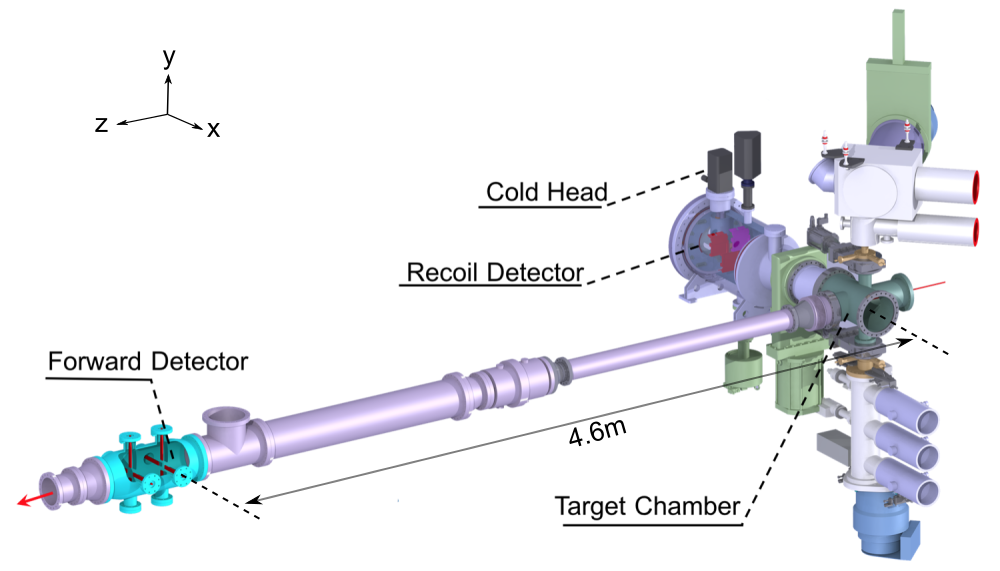
\includegraphics[width=0.9\textwidth]{./koala_setup.png}
\caption{3D visualization of the KOALA setup at COSY}
\label{fig:setup}
\end{figure}

The hydrogen cluster target connects vertically to the target chamber, with the target generator on the top and the target beam dump on the bottom.
The recoil arm is located on the \(-X\) axis. The recoil chamber holds the recoil detector, which is installed about \(1m\) from the interaction point.
One gate valve is installed between the target chamber and the recoil chamber. 
It is used for staged pumping of the recoil chamber during the preparation of the experiment, protecting the recoil sensors from the beam residual gas.
The forward arm overlaps with the beam pipe. The forward chamber connects to the target chamber through one \(\diameter 90\) mm pipe and one \(\diameter 200\) mm pipe. 
The forward detector is installed inside the forward chamber, which is located about 4.6 m away from the interaction point.

The hydrogen cluster target is upgraded from the old ANKE target \cite{cluster_target}.
A new collimator is installed to provide a much smaller width of the cluster beam on the beam axis, which is measured to be about 2 mm.
The areal density of the cluster beam is estimated to be \(10^{14}\) \(atoms/cm^2\).
A windowless target with low material budget and thin thickness is critical in KOALA.
The energy loss of the recoil proton before hitting the recoil sensor should be minimized to get an accurate measurement of the kinematic energy.
And the spread of the interaction position should be minimized so that the distortion of the energy spectrum is negligible. 

\section{Recoil detector}
\label{sec:recoil}

\begin{figure}[htbp]
\centering
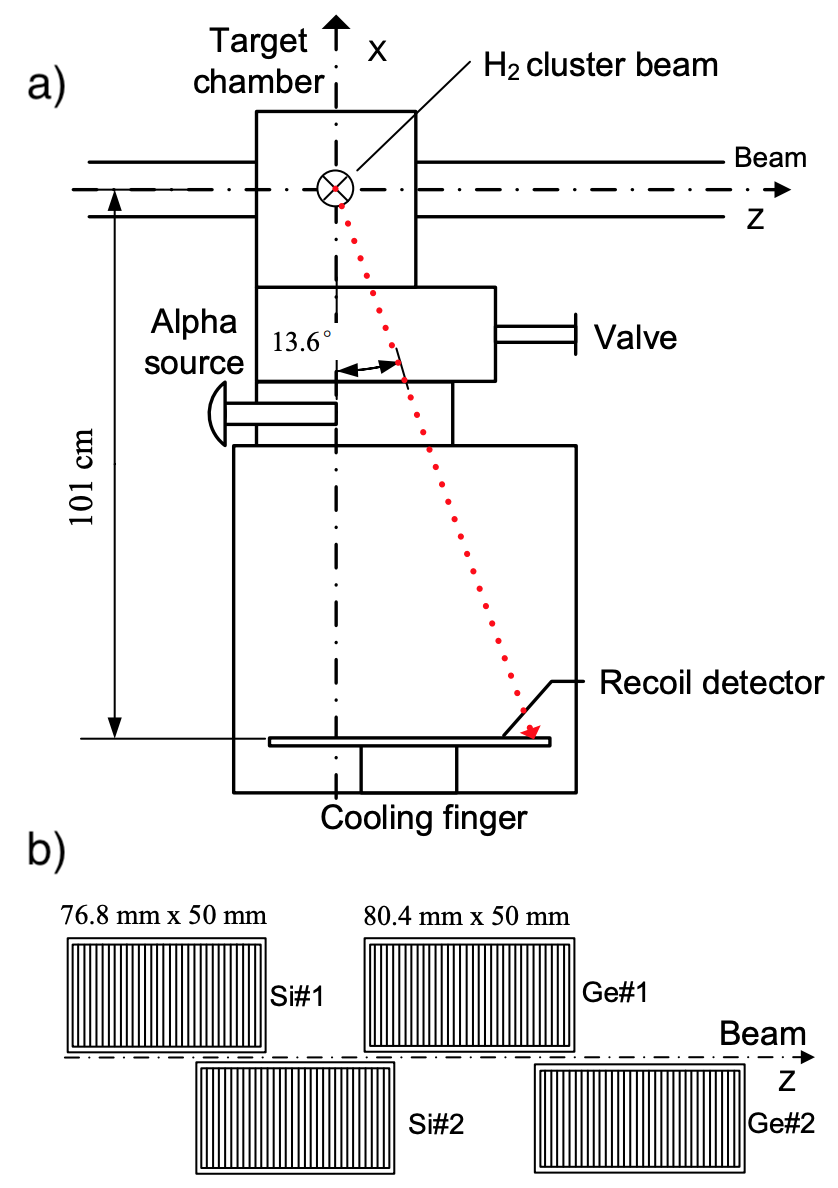
\includegraphics[width=0.9\textwidth]{./recoil_schematic.png}
\caption{(a) A schematic view of the recoil detector; (b) Layout of the four sensors}
\label{fig:org9ed7981}
\end{figure}

The recoil detector of KOALA needs to stop the recoil proton from the elastic scattering and measures the hit position and the total energy loss.
It needs to cover a large dynamic range of recoil energy required by KOALA design.
For elastic scattering process of two particles with the same mass,
the value of \(|t|\) is proportional to the kinematic energy of recoil proton \(T_p\) by \(|t| = 2m_pT_p\), where \(m_p\) is the proton mass.
\(|t|=0.1\) \((GeV)^2\) corresponds to \(T_p \approx 54\) MeV. 
This means solid state sensors with modest thickness can be used to fully stop the recoil proton. 
Position-sensitive solid state sensors are ideal in this case, since they provide excellent energy resolution.

The recoil detector consists of two single-sided silicon strip sensors and two single-sided germanium strip sensors with a layout shown in Fig. \ref{fig:org9ed7981} (b).
The sensors are arranged along the beam axis with staggered placement in the Y-axis.
Sensors at different recoil angle have different thickness: 1 mm for Si\#1 and Si\#2, 5 mm for Ge\#1, 11 mm for Ge\#2.
The silicon sensors have an sensitive area of \(76.8 \times 50\) mm, which are segmented into 64 strips of 1.2 mm width.
The germanium sensors have an sensitive area of \(80.4 \times 50\) mm, which are segmented into 67 strips of 1.2 mm width.
Neighboring sensors have a small overlapping region which is symmetric against the beam axis.
The strips in the overlapping region are used for sensor alignment and beam position correction.
The four sensors form a detection plane, which is about 1 m away from beam-target overlapping center.

The sensors are readout by a combination of the charge-sensitive preamplifier (MPR16 for the strips, MPR1 for the rear side) 
and the timing filter amplifier (MSCF16), both from Mesytec \cite{mesytec}. 
MSCF16 integrates the shaping amplifier and leading-edge discriminator in the same module.
Both amplitude and timing signal are extracted from MSCF16 for energy and time measurement.
Strips at large recoil angle and unphysical region can be combined into a single readout channel without sacrifice of the angular resolution.
In total, there are 180 readout channels for the recoil detector: 
48 channels on Si\#1, 64 channels on Si\#2, 32 channels for Ge\#1 and Ge\#2, 4 channels for the rear side. 

The temperature of the four sensors is monitored by four PT100 temperature sensors.
The working temperature can be adjusted by a combination of the cold head and two heating resistors on the cold plate.
The adjustment is controlled actively by a high-precision Lake Shore Model 336 temperature controller.
A study of the performance of recoil sensors in the laboratory shows that the optimal working temperature is about 125 K.
Under this condition, the energy resolutions of the silicon and germanium sensors are better than 20 keV and 30 keV (FWHM) respectively.

More detailed information about the recoil detector can be found in \cite{recoil_article}.

\subsection{Energy calibration}
\label{sec:calibration}

Precise determination of energy deposit in the recoil detector is crucial for the identification of elastic scattering events and the calculation of the recoil angle.
\(\alpha\) sources \(^{239}Pu\), \(^{244}Cm\), \(^{241}Am\) are used for the energy calibration, with main decay energies of 5156.59 keV, 5804.83 keV, 5485.56 keV \cite{nuclear_data} respectively.
Other decay modes with much smaller branch ratios also exist. They may also be used in the energy calibration if they are well separated from the main peaks.
The alpha sources are mixed and installed on a linear motion feedthrough rod.
During experiment, the rod is lifted and the sources are blocked by the chamber wall;
during calibration, the rod is pushed to the chamber center and the sources face the recoil sensors directly.
Thus, the recoil detector can be calibrated regularly after commissioning.

Two aspects need special consideration in the calibration. Firstly, the recoil sensors have a protective layer on the surface. 
\(\alpha\) particles lose a small fraction of their energy in this layer before entering the fiducial volume.
The thickness of the protection layer has already been measured in the laboratory using \(\gamma\) rays \cite{recoil_article}.
The energy loss in the protection layer is calculated and shown in Tab. \ref{tab:dead_layer} for each $\alpha$ energy when the incidence angle in $90\degree$.
The effective energy deposit in the fiducial volume is further corrected based
on the recoil angle of each strip.

\begin{table}[htbp]
\label{tab:dead_layer}
\caption{Energy loss (keV) of $\alpha$ in the protection layer when incidence angle is $90\degree$}
\centering
\begin{tabular}{cccccc}
\hline
\(E_{\alpha} (keV)\) & \(\Delta E_{Si1}\) & \(\Delta E_{Si2}\) & \(\Delta E_{Ge1}\) & \(\Delta E_{Ge2}\) \\
\hline
5156.59 & 11.51 & 11.51 & 110.00 & 111.00 \\
5485.56 & 11.01 & 11.01 & 105.00 & 106.00 \\
5804.83 & 10.52 & 10.52 & 99.00  & 100.00 \\
\hline
\end{tabular}
\end{table}

Secondly, the gain setting of each readout channel is optimized for the covered energy range at its recoil angle.
The gain difference between different channels varies up to a factor of 10.
Thus, the separation of the energy peaks is much smaller at large recoil angle than at small recoil angle, as shown in Fig. \ref{fig:alpha_spectrum}.
The minor peaks can't be recognized in Fig. \ref{fig:alpha_spectrum} (a), while they are clearly separated in Fig. \ref{fig:alpha_spectrum} (b).
Smaller separation brings larger systematic error in the calibration.

\begin{figure}[htbp]
\centering
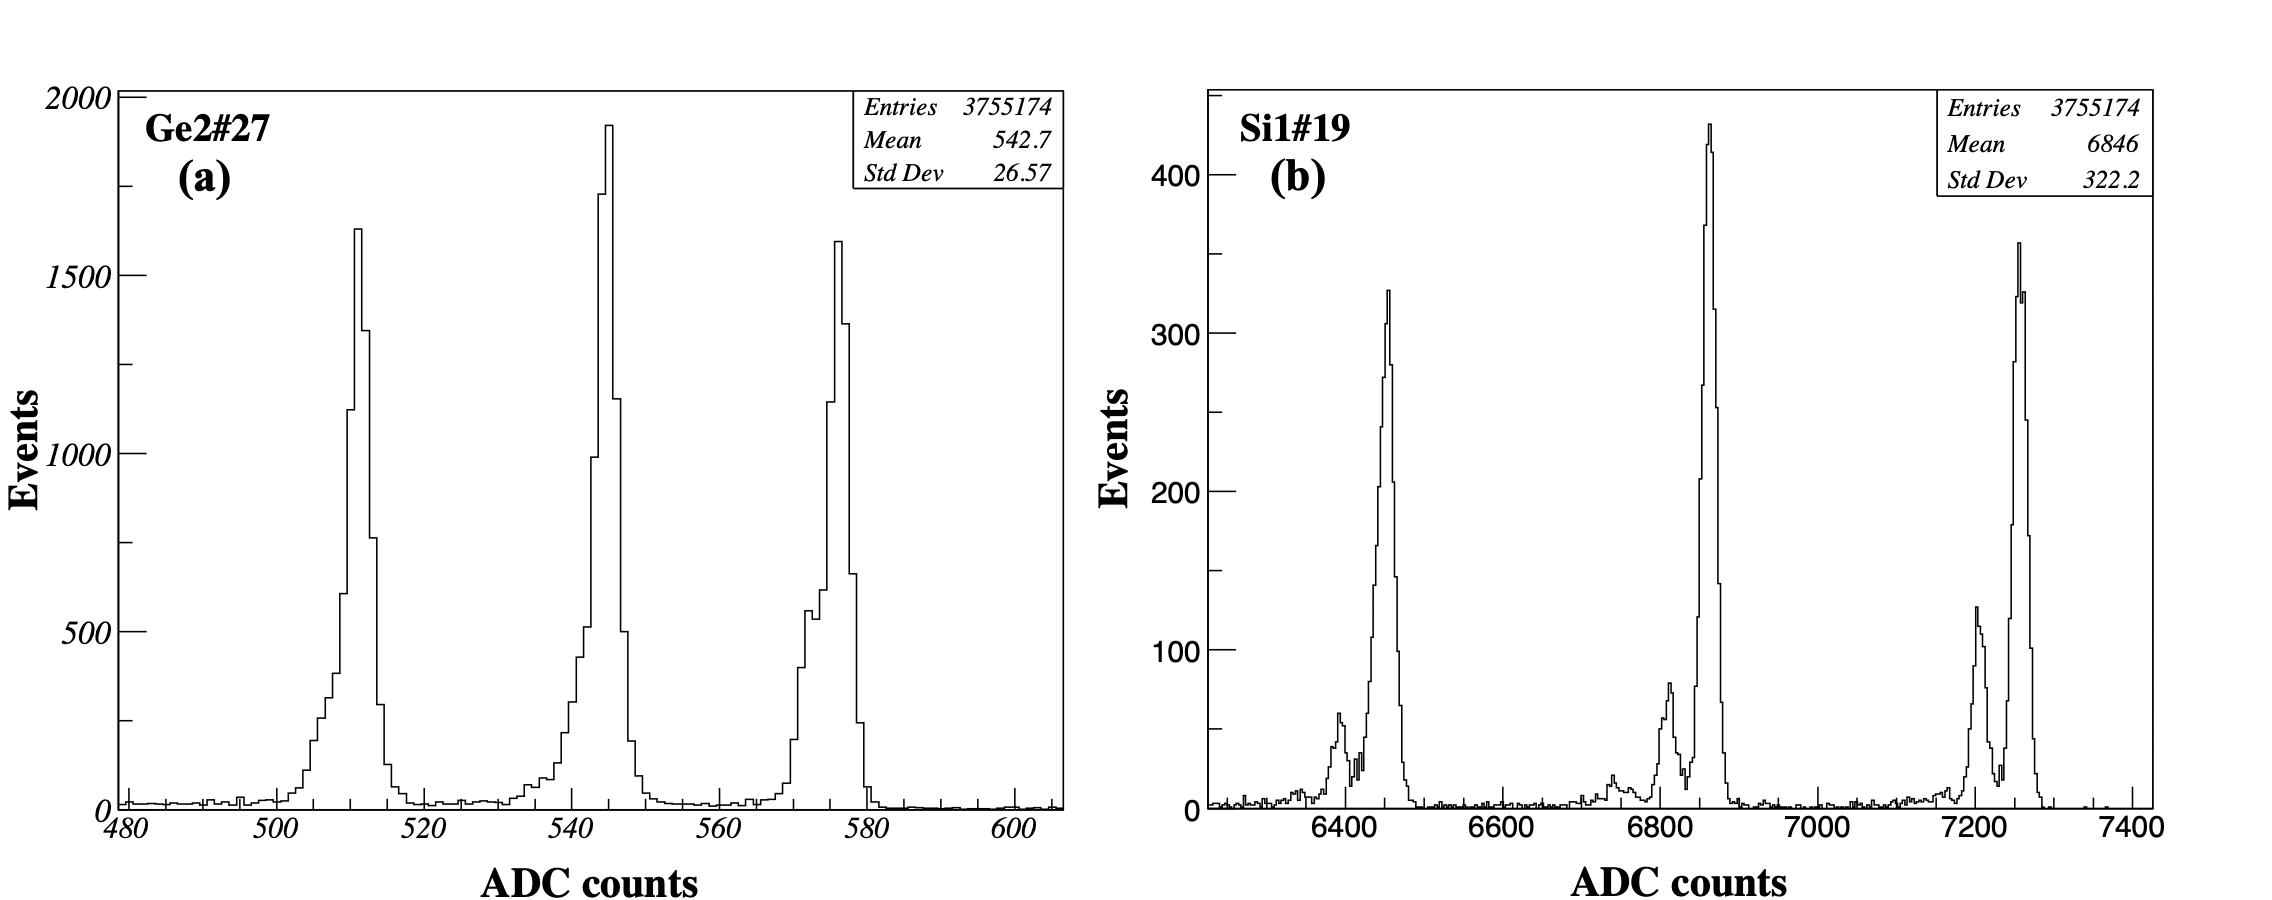
\includegraphics[width=0.9\textwidth]{./alpha_response.png}
\caption{Energy spectrum of \(\alpha\) sources of two channels at different recoil angles: (a) small recoil angle; (b) large recoil angle}
\label{fig:alpha_spectrum}
\end{figure}

\begin{figure}[htbp]
\centering
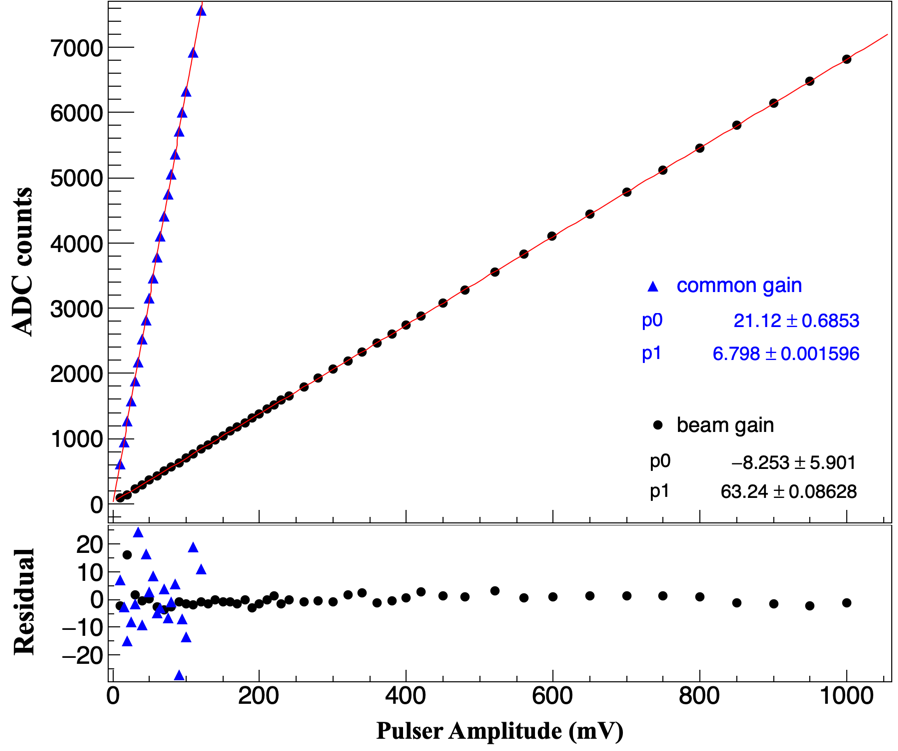
\includegraphics[width=0.9\textwidth]{./linearity.png}
\caption{Electronic linearity of a typical recoil detector channel}
\label{fig:electronic_linearity}
\end{figure}

To minimize this error, a common gain, which is optimized for the separation of the \(\alpha\) energy peaks, is set for all channels.
Then, the calibration is carried out as follows:
\begin{enumerate}
\item the energy spectrum of the \(\alpha\) sources is recorded under the common gain setting and the peaks of \(\alpha\) enegies are searched;
\item the gain difference between the common gain and the actual gain setting in the beam test is measured by scanning a precision analog pulser over a large range of amplitudes;
\item the actual energy responses are deduced by applying the gain difference to the common gain responses, and the result is fitted using a linear function.
\end{enumerate}
The fitting parameters of the last step are the parameters used to convert ADC values into energy values in reconstrunction.

The electronics of recoil detector have very good linearity in the dynamic range needed by KOALA.
A typical example is shown in Fig. \ref{fig:electronic_linearity}. 
Thus, the systematic error of this indirect method of energy calibration is very small.

\subsection{Time-walk correction}
\label{sec:timewalk}

\begin{figure}[htbp]
\centering
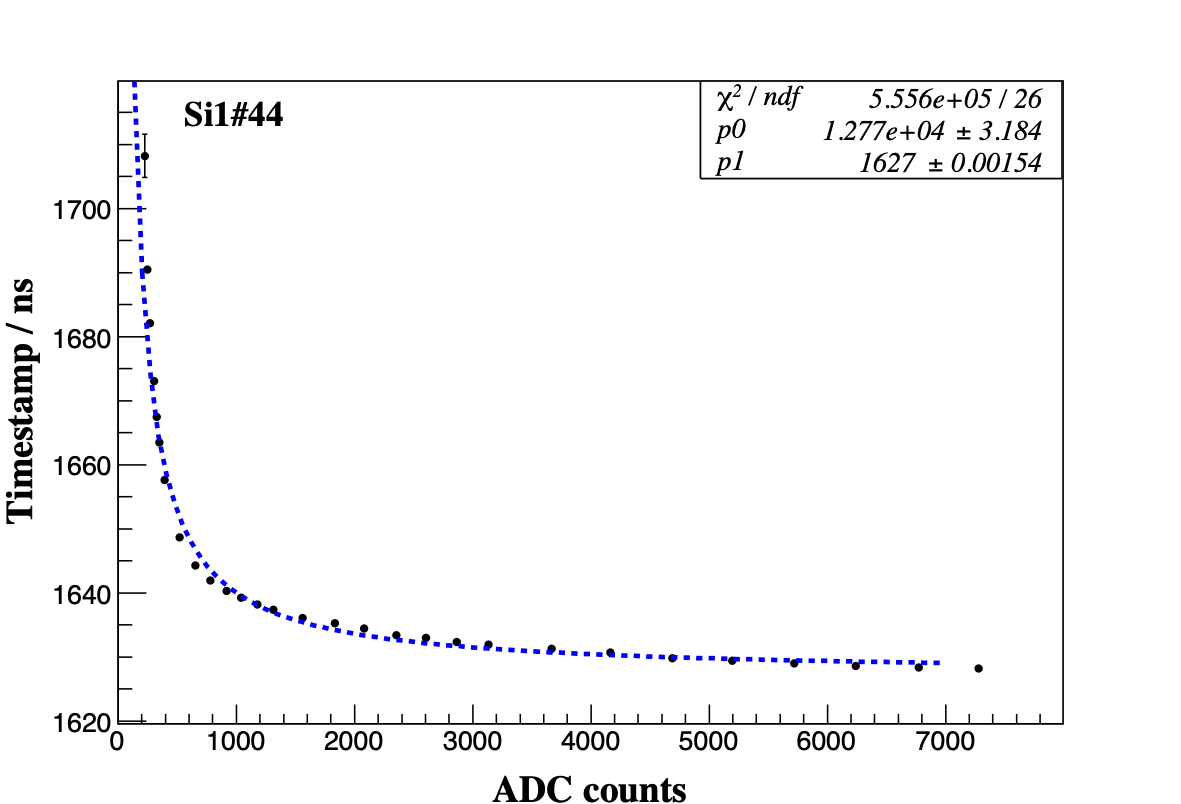
\includegraphics[width=0.9\textwidth]{./timewalk.png}
\caption{Typical result from the time-walk calilbration.}
\label{fig:timewalk}
\end{figure}

Time-walk effects of the leading edge discriminator need to be corrected offline to get accurate time information.
Calibration of the time-walk effect is carried out using a  precision analog pulser. 
Output from the pulser is split into two branches. One is fed into a constant fraction discriminator to generate the trigger signal for DAQ, 
the other is connected to the detector channel for measurment. 
By scanning the pulser over a wide range of amplitudes, the time-walk effect is revealed as shown in Fig. \ref{fig:timewalk}.
The result is fitted using \(y=p_0 x^{-1} + p_1\). 
\(\Delta T = p_0 \cdot ADC\) is the correction value for the time-walk effect.
\(p_1\) difference between detector channels indicates the delay time difference, which in turn reveals the signal routing length variation.
These offset values are used to align the timestamps from different channels in the reconstrunction.

\section{Forward detector}
\label{sec:fwd}

The forward detector aims to measure the arrival time of the scattering proton over the region \(0.0005 < |t| < 0.004\) \((GeV/c)^2\).

The forward detector consists of 8 detector modules which are grouped into 4 pairs. The modules in the same pair are separated by 20 cm.
These 4 pairs are installed symmetrically around the beam pipe center as shown in Fig. \ref{fig:setup}.
The first layter of the detector modules are placed 4.6 m downstream the beam-target overlapping center.
In principle, only the pair on +X axis is needed for the detection of the scattering proton. 
The other 3 pairs are used for beam position monitoring during experiment.

Plastic scintillator BC-408 \cite{bc408} is selected as the sensor material due to its good timing performance (0.9 ns rise time).
Each forward detector module consists of one piece of square BC-408 with dimension \(90 (length) \times 20 (width) \times 6 (thickness)\) mm.
The scintillator is coupled to a PMT (Hamamastu H6900 \cite{hamamatsu}) with a tapered light guide and a silicone pad.
The forward detector modules are integrated with the forward chamber flange and  installed 3 cm away from the beam center.
This indicates an acceptance of scattering angle \(0.4\degree < \theta < 1.5\degree\).
To protect the ultra-high vacuum condition, minimum material budget principle is implemented in the design of the detector module:
\begin{enumerate}
\item only the light guide and the scintillator are located inside the forward chamber, the light guide is glued on the open port of the flange as a feedthrough;
\item no wrapping and painting material on the surface of the scintillator, the surface is polished to increase light collection efficiency;
\item a thin aluminum tube with thickness of \(100 \mu m\) is used as the light shield of the scintillator, the tube is welded on the flange (Fig. \ref{fig:forward_module} (a);
\item two small holes are opened on the side of the aluminum tube to speed up vacuum pumping.
\end{enumerate}
Components like silicone pad, PMT, PMT base are installed in a light-tight box on the other side of the flange as shown in Fig. \ref{fig:forward_module} (b).

\begin{figure}[htbp]
\centering
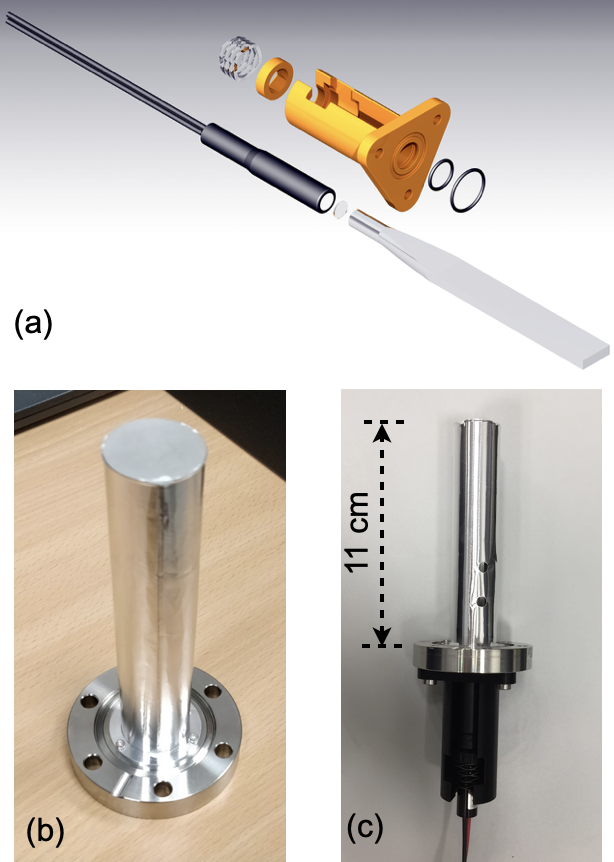
\includegraphics[width=0.9\textwidth]{./forward_module.png}
\caption{(a) The aluminum tube is welded on the inside of the flange; (b) One forward detector module after complete assembly}
\label{fig:forward_module}
\end{figure}

\begin{figure}[htbp]
\centering
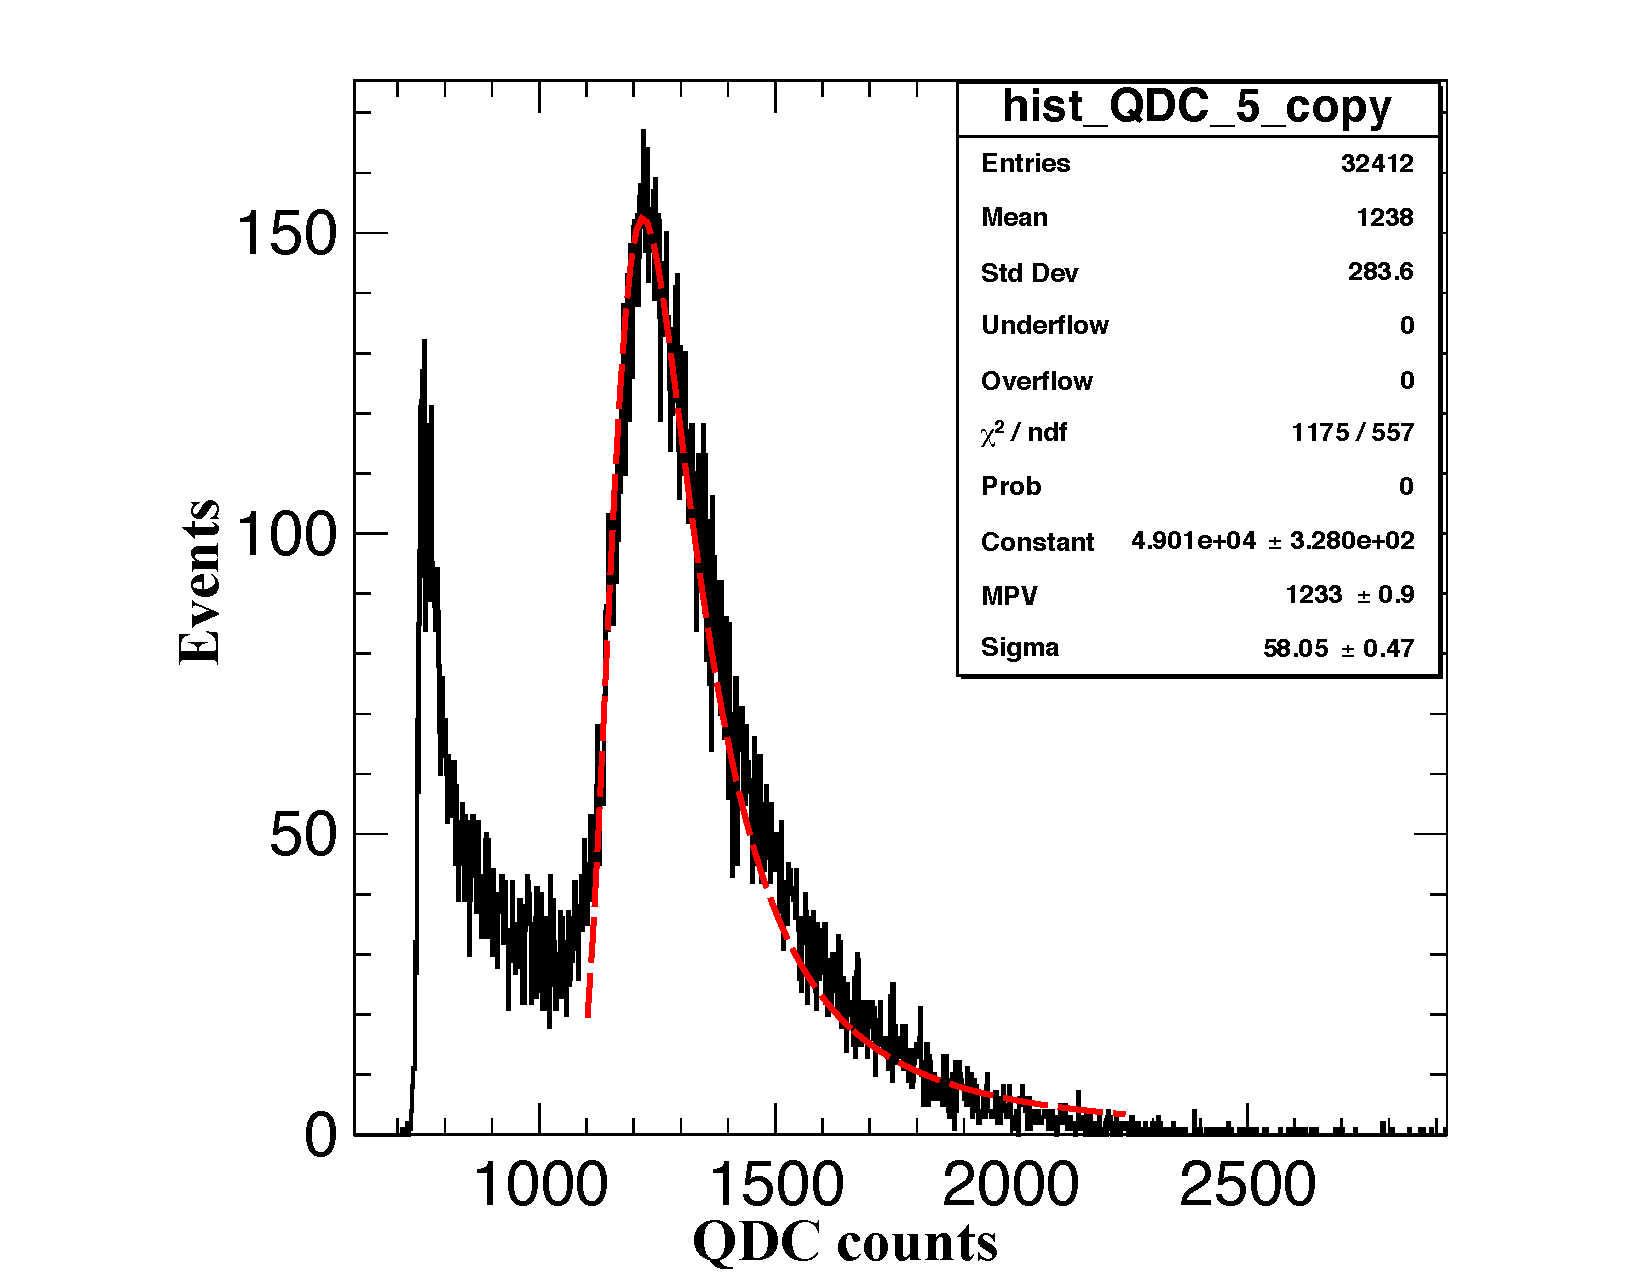
\includegraphics[width=0.9\textwidth]{./forward_mip.pdf}
\caption{An example of the cosmic ray energy spectrum obtained by a forward detector module prototype}
\label{fig:forward_mip}
\end{figure}

Due to the large amplitude of the output signal, no front-end electronics is needed for the readout of the forward detector.
The output signal from PMT is split into two branches: one connecting to the CF discriminator for time information extraction; the other for charge measurement directly.
A typical MIP spectrum obtained by the forward detector module using cosmic ray is shown in Fig. \ref{fig:forward_mip}. 
The MIP peak is clearly separated from the pedestal noise, with signal to noise ratio better than 50.
The timing resolution is about 140 ps.
the
\section{Data acquisition system}
\label{sec:daq}

The data acquisition system of KOALA is a VME-based system with multiple types
of digitization modules provided by Mesytec \cite{mesytec}.
For the recoil detector, the amplitude signal from MSCF16 is digitized by a peak-sensing ADC called MADC-32.
MADC-32 has a 13-bit dynamic range with 6.4 \(\mu s\) conversion time.
For the forward detector, the pulses from PMT are directly fed into a QDC called MQDC-32 for charge measurement.
MQDC-32 has a dynamic range of 500 pC and it uses a 12-bit ADC for digitization with 250 ns conversion time.
The timing information from both the recoil and forward detectors are recorded by the TDC module called MTDC-32 using a conventional Start-Stop method.
MTDC-32 has a minimum resolution of 5 ps.
A multi-channel scalar called SIS3820 \cite{sis} is also integrated to measure the following key count rates: 1) count rates of all the four arms of the forward detector for 
beam position monitoring; 2) count rates of the overlapping strips of the recoil detector for asymmetry correction; 3) count rates of the input trigger
for DAQ efficiency correction.
The VME controller is SIS3100 from Struck Innovative \cite{sis}.

The acceptance of the forward detector only covers a small part of the recoil detector sensors.
To record the elastic scattering events from the whole range of the recoil angle covered by the recoil detector, KOALA adopts a self-triggering schemde for the trigger logic design.
Each sensor of the recoil detector and each arm of the forward detector works independently and generates their own trigger. 
The trigger of the DAQ system is a common OR of the sub-detectors, as shown in Fig. \ref{fig:trigger_logic}.
The trigger from the recoil detector sensor is generated by a coincidence between the front-side strips and the rear-side plane, 
and the trigger from the forward detector arm is generated by a coincidence between the two layers in the same pair.
In this way, the rate of the false hits generated by electronic noise can be minimized.
Both elastic and inelastic scattering events are recorded in a self-triggering mode, and the coincidence between the recoil sensor and the forward detector is carried out in an offline analysis.

\begin{figure}[htbp]
\centering
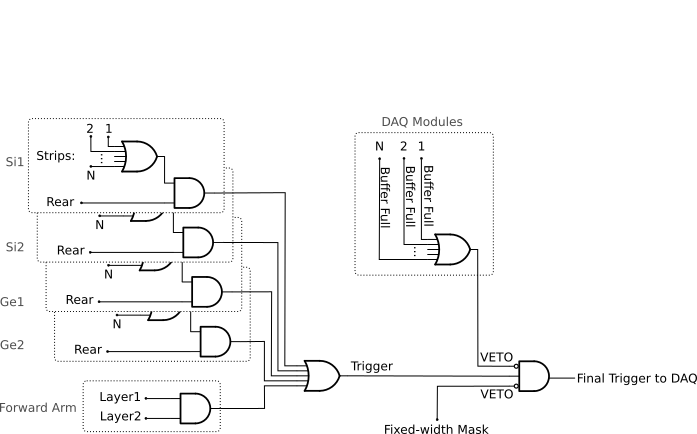
\includegraphics[width=0.9\textwidth]{./trigger_logic.png}
\caption{Trigger Logic of the KOALA DAQ.}
\label{fig:trigger_logic}
\end{figure}

Fast readout of the recorded event is crucial for a self-triggered DAQ system.
The asynchronous readout mechanism is adopted to increase the data throughput in KOALA.
Each digitization module in the system has an on-board event buffer with a minimum size of 32 kB.
The newly-digitized event is stored in this buffer before readout, so that the
module is immediately ready for the digitization of the next event.
The events in this buffer are not readout until the buffer is nearly full. In
this way, the readout and the digitization is decoupled in order to minimize dead time of the module.
Furthermore, VME CBLT transfer mode is utilized to minimize protocol overhead and in turn improve the readout speed.
Since the hit rate is much higher at small recoil angles, the event buffer for these channels always saturates faster than others.
Modules with a saturated event buffer will not record any new coming events before readout of the recorded events, while other modules are still able.
This will bring a underestimated event counts in the region with smaller recoil angles.
To solve this problem, the buffer-full flag signal from each digitization
module is added to the trigger logic as a VETO as shown in Fig. \ref{fig:trigger_logic}.

The issue about event synchronization arises naturally when using asynchronous readout.
The digitization modules used in KOALA have different dead time, especially between MADC-32 and MTDC-32.
An event recorded by a fast module may be missed by a slow module. This creates un-synchronous event structure, which makes the sequential event data assembling impossible. 
KOALA DAQ uses timestamp-based synchronization to solve the problem.
The modules in the system all have a 30-bit timestamp counter to record an input clock signal from the same source.
The central clock source can be either the VME built-in clock of 16 MHz or an external clock to up 75 MHz.
Currently, the built-in clock of VME backplane bus is used. 
Based on this timestamp, event synchronization is achieved offline.
An alternate option is to introduce a fixed-width mask signal into the trigger logic as VETO, as show in Fig. \ref{fig:trigger_logic}.
The width of the mask signal should be larger than the largest dead time of all modules.
In this way, the events are effectively synchronized sequentially. 
However, this may also reduces DAQ efficiency significantly in a high hit-rate environment, which is not preferred.

\begin{figure}[htbp]
\centering
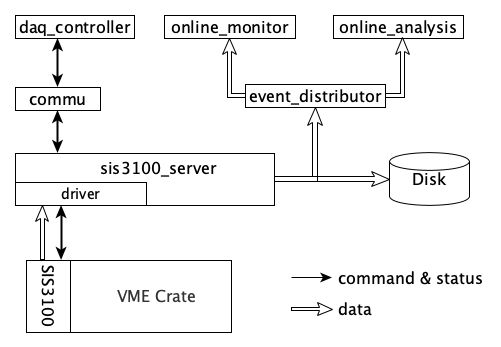
\includegraphics[width=0.9\textwidth]{./koalaems_deployment.png}
\caption{Design and deployment of KoalaEms.}
\label{fig:koalaems}
\end{figure}

A dedicated DAQ software called KoalaEms is also developed for KOALA.
KoalaEms is a fork of the EMS software \cite{ems}, which is a highly flexible DAQ software framework developed for various experiments previously conducted at COSY.
Support for the SIS3100 controller is integrated into KoalaEms and a new component of online monitoring based on ROOT is added.
Also, outdated and unused components are updated and removed, respectively.
The design of KoalaEms and the topology of deployment are shown in Fig. \ref{fig:koalaems}.
The interface to DAQ is implemented as \emph{sis3100\_server}, the host PC of which has an optical link to the VME crate.
The command and status information from/to the \emph{daq\_controller} is mediated by a component called \emph{commu}.
The data flow from VME crate have two branches: 1) \emph{data\_out\_disk}: save the raw data onto disk; 2) \emph{data\_out\_stream}: stream out to \emph{event\_distributor} for dispatching.
\emph{event\_distributor} will in turn forward the data stream to various consumption hosts for usages like online monitoring or online analysis.
Both \emph{commu} and \emph{event\_distributor} support socket connection and the \emph{event\_distributor} also supports multiplexing streaming.
Thus, all the square blocks in Fig. \ref{fig:koalaems} can be hosted in different PCs and new consumer host to the data stream can be integrated when needed.


\section{Software framework}
\label{sec:software}

A dedicated software framework called KoalaSoft is developped for the simulation, calibration, reconstrunction and analysis jobs of the KOALA experiment.
It is built upon the FairRoot \cite{fairroot} framework, which implements a simulation environment based on VMC \cite{vmc} library and an analysis environment based on ROOT's task concept.
The components stack of KoalaSoft is shown in Fig. \ref{fig:koalasoft}.

\begin{figure}[htbp]
\centering
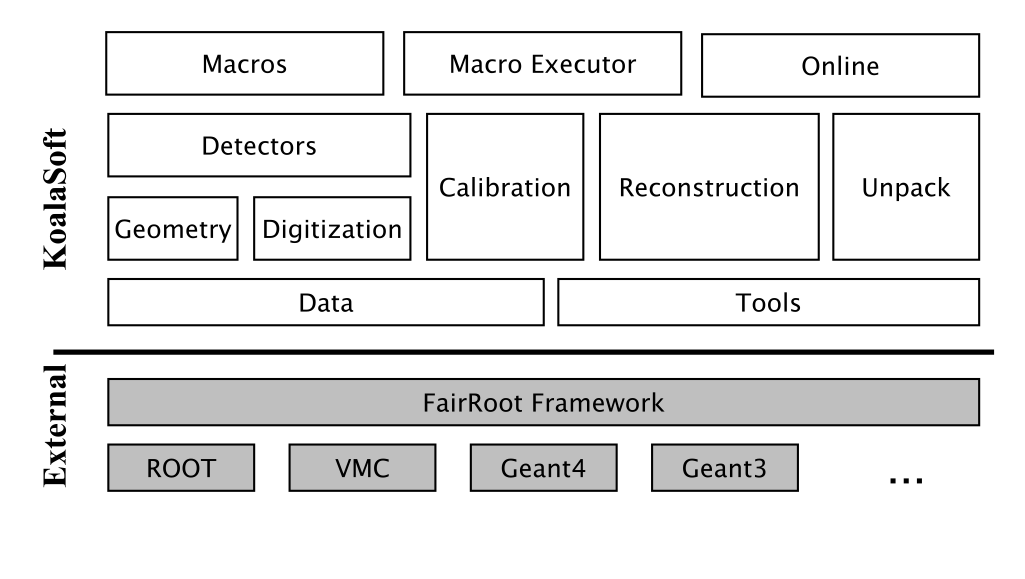
\includegraphics[width=0.9\textwidth]{./koalasoft_components.png}
\caption{Components of KoalaSoft}
\label{fig:koalasoft}
\end{figure}

Both Geant3 and Geant4 can be selected as the simulation engine without changing other components in KoalaSoft.
Geometry models of the recoil detector and the forward detector are implemented using ROOT's TGeo library.
Jobs like digitization, calibration and reconstrunction are divided into multiple smaller steps, each of which is represented by a single task.
Tasks are selected and chained together later in a ROOT macro to compose a meanful job. 
ROOT macros are the interface for the end user using KoalaSoft.
Macros for common jobs are pre-configured and distributed along with KoalaSoft.
End users are also free to compose their own specific jobs for analysis.
Additionally, a binary macro executor is provided to run jobs directly from command line. This may be useful in batch processing.

In KoalaSoft, the same chain of tasks can be used for the analysis of both the simulation data and the raw data from DAQ.
This is accomplished by the \emph{Unpack} component, which can decode and transform the raw binary data into the same format as the output from simulation jobs.
The feature allows that the algorithms developped, tested and verified using simulation data be applied to experimental data seamlessly.
This saves a lot of efforts in the development and maintainence of algorithms.
Both the offline disk data and the online streaming data are correctly handled by \emph{Unpack} and an online monitoring program is developped based on it.

\section{Test beam results}
\label{sec:result}

\begin{figure}[htbp]
\centering
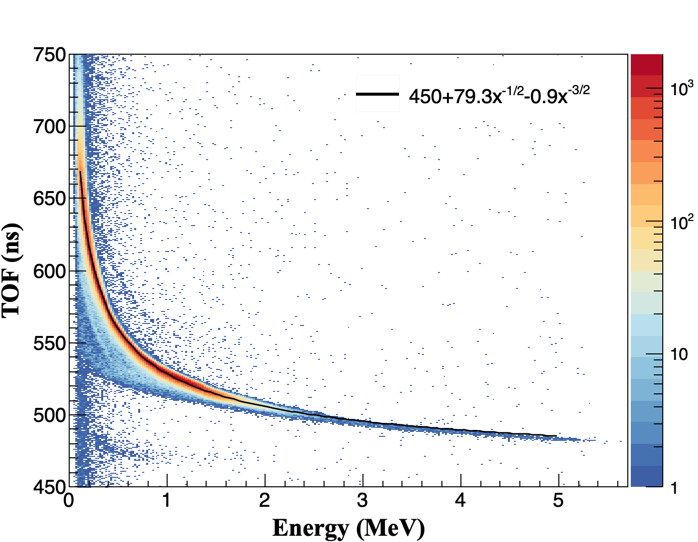
\includegraphics[width=0.9\textwidth]{./tof_e_cut.png}
\caption{
Typical TOF-E spectrum of recoil proton recorded at beam energy 2.6 GeV/c. Here, \textbf{TOF} is the time difference between the timestamp from recoil sensor and forward detector. \textbf{E} is the energy recorded by recoil sensor. The data is from recoil strips covered by forward detector.}
\label{fig:tof-e}
\end{figure}


\begin{figure}[htbp]
\centering
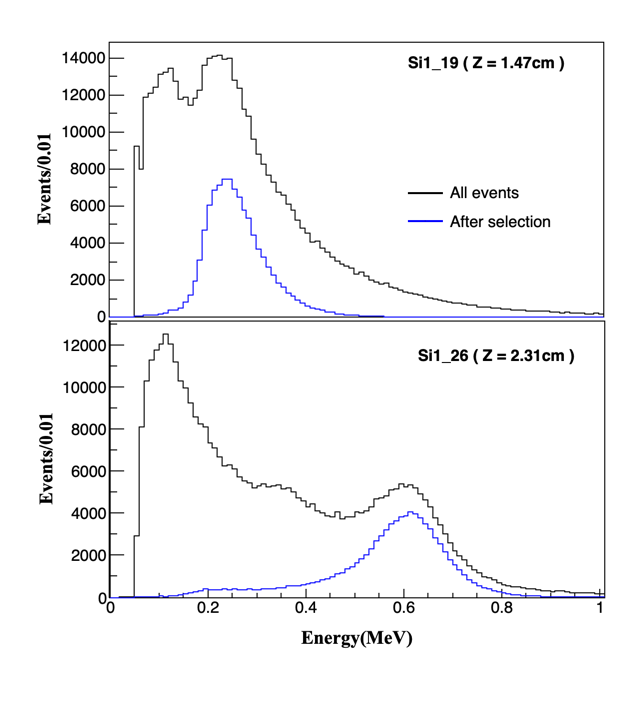
\includegraphics[width=0.9\textwidth]{./comparison_tof_e_cut.png}
\caption{Energy spectrum of Si1\_16 before (black) and after (blue) TOF-E cut.}
\label{fig:cut}
\end{figure}

\begin{figure}[htbp]
\centering
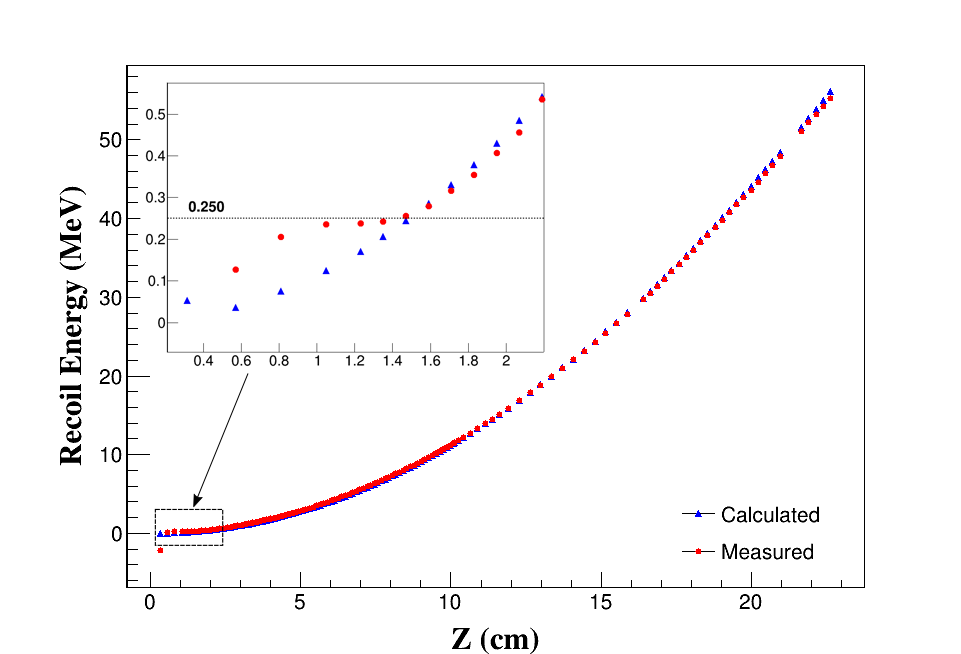
\includegraphics[width=0.9\textwidth]{./calc_vs_measured_combined.png}
\caption{
Comparison of measured (red circle) and calculated (blue triangle) recoil energy with respect to strip position along z-axis (i.e. beam direction). Beam energy is 2.6 GeV/c.}
\label{fig:measured_vs_calculated}
\end{figure}

The verification of the full KOALA setup with the new forward detector and the updated components was carried out using proton-proton elastic scattering with beam energy
2.2, 2.4, 2.6 and 3.0 GeV/c.

The coincidence between the recoil detector and the forward detector was observed clearly in these tests.
A typical result of TOF-E spectrum from the recoil protons is shown in Fig. \ref{fig:tof-e}. 
The elastic scattering events are distributed as the major band in the middle of the graph, which can be fitted with the relation \(TOF = p_{0} + p_{1}/{\sqrt{E}}\).
The events lying outside of the major band are from inelastic scattering process and they will overlap with the elastic events at small recoil angles when projected to the energy spectrum.

To select the elastic events, the fitting result of the TOF-E major band is moved up and down to form a cut region as shown in the pink curves in Fig. \ref{fig:tof-e}.
A typical result after applying the TOF-E cut is shown in Fig. \ref{fig:cut}.
The elastic peak is filtered out from a large background after the cut and a more accurate fitting can be applied in the new spectrum.

Applying this method to all strips covered by the forward detector, the lowest measurable energy, i.e. the smallest |t|, is deduced.
Fig. \ref{fig:measured_vs_calculated} shows the comparison between the measured energy peak and the expected energy of recoil proton from elastic scattering at 2.6 GeV/c.
A limit is observed around \(250 keV\), which corresponds to |t| approximately 0.0005 \((GeV/c)^2\).

\section{Conclusion}
\label{sec:conclusion}

The commissioning of the KOALA setup at COSY, specifically the new forward detector, is successful.
A strong correlation between the recoil detector and the forward detector is observed for elastic scattering events at small |t|.
The TOF-E relation of the recoil proton from elastic scattering can be used to effectively suppress the large background events.
The designed |t| range of KOALA are achieved with this setup.

The updated DAQ operates in stable condition in all tests.
The maximum recorded rate is about $\%10^3$ events/s, with an efficiency of 96\%.
Limited performance of DAQ may bring efficiency bias in different sub-detectors.
Optimization of the DAQ is possible by removing the gate mask in the trigger logic.
In this case, more tests of the timestamp-based synchronization in the offline analysis are needed.

\bibliographystyle{elsarticle-num}
\bibliography{reference}

\end{document}
